\documentclass[runningheads]{llncs}
\usepackage{graphicx}
\usepackage{url}
\renewcommand{\refname}{Referinte}

\begin{document}
\title{\huge{Analiza Algoritmilor\\Tema - Etapa 3}}
\author{\textit{\large{Grigore Lucian-Florin}}}
\institute{\textit{\large{Grupa 324CD\\Facultatea de Automatica si Calculatoare\\Universitatea Politehnica, Bucuresti}}}
\maketitle              
\begin{abstract}
Acest document reprezinta forma finala a studiului realizat asupra algoritmilor de pattern-matching Knuth-Morris-Pratt si Rabin-Karp.

\keywords{Rabin-Karp \and Knuth-Morris-Pratt \and Pattern-Matching.}
\end{abstract}

\section{Introducere}
\subsection{Descrierea problemei rezolvate}
\paragraph{} Problema abordata presupune gasirea celei mai lungi secvente comune pentru doua siruri de caractere - \textit{pattern-matching}.

\subsection{Exemple de aplicatii practice pentru problema aleasa} 
\paragraph{} Conceptul de pattern-matching are multiple aplicatii in domeniul calculatoarelor, unele dintre cele mai interesante fiind:
\begin{enumerate}
\item Procesarea limbajului natural
\item Motoarele de cautare web
\item Detectarea si combaterea intruziunilor cibernetice
\item Citirea si interpretarea biosecventelor din ADN
\item Gestionarea pachetelor de internet de catre routere
\end{enumerate}

\subsection{Specificarea solutiilor alese}
\paragraph{} Solutiile alese pentru rezolvarea acestei probleme sunt algoritmii Rabin-Karp (Michael Rabin si Richard Karp) si Knuth-Morris-Pratt (James H. Morris, Donald Knuth si Vaughan Pratt).

\subsection{Specificarea criteriilor de evaluare alese pentru validarea solutiilor}
\begin{itemize}
		\item Pentru \textbf{Rabin-Karp}, dorim sa gasim probabilitatea unei false potriviri in functie de dimensiunea spatiului cheilor, precum si folosirea mai multor tipuri de functii hash in implementare (eficiente si mai putin eficiente). In schimb, se pot elimina foarte usor secventele care nu se potrivesc cu ajutorul unei functii hash potrivite. Pe de alta parte, se poate slabi performanta algoritmului foarte mult daca este folosite o functie de hashing slaba. Ne intereseaza gasirea unei functii de hashing cat mai \textit{fail-proof} pentru o performanta mai buna.
	\item Cazurile cand algoritmul \textbf{Knuth-Morris-Pratt} functioneaza mai bine decat Rabin-Karp, si invers.
	\item \textbf{Complexitatile} de timp si spatiu ale fiecarui algoritm pentru un set de date de dimensiune cunoscuta \textit{(cea mai lunga secventa fiind de o lungime M, cunoscuta)}.
	\item Dorim sa intocmim un \textbf{set de teste} care sa se asigure ca solutiile propuse functioneaza cat mai eficient din punctul de vedere al memoriei si timpului de executare. Testele propuse ar trebui sa acopere situatii precum: potrivirea multipla intre secvente de aceeasi lungime (preferabil lungime mare, pentru a vedea consumul resurselor), secvente care sa para la fel pentru functii hash slabe (de exemplu "aab" si "aba" ar avea aceeasi valoare hash pentru o functie care nu se foloseste de indexul literelor) sau secvente cu grupuri de litere repetitive care sa puna la incercare tabela caracteristica algoritmului KMP.
\end{itemize}

\section{Prezentarea solutiilor}
\subsection{Descrierea modului in care functioneaza algoritmii alesi}
\paragraph{} Algoritmul \textbf{Rabin-Karp} este la baza \textit{bruteforce} la care se adauga o componenta foarte puternica in programare, si anume \textit{hashingul}. Nu este folosit asa mult la scara larga deoarece are o complexitate de timp slaba. Pe de alta parte, el prezinta avantajul ca isi mentine complexitatea indiferent de numarul de match-uri din text.
\paragraph{} Folosirea hashingului are rolul de a creste eficienta acestei solutii prin exploatarea aspectului ca doua siruri egale au aceeasi valoare de hash. Un dezavantaj al acestei abordari este acela ca se pot potrivi ca valoare hash doua siruri care nu sunt identice. Din aceasta cauza acest algoritm presupune si verficarea (caracter cu caracter) a celor doua siruri care au aceeasi valoare hash pentru a asigura potrivirea lor.
\paragraph{} Pasii de realizare ale acestei solutii sunt: \\
\begin{itemize}
\item calcularea valorii hash a pattern-ului
\item calcularea valorii hash a primelor m caractere din text (unde m este lungimea pattern-ului)
\item compararea celor doua valori hash. Daca sunt egale, ori se termina executia functiei, ori se adauga pozitia pe care a fost gasit pattern-ul in text intr-o lista de indici
\item in cazul unei nepotriviri, se recalculeaza noua valoare hash a urmatoarelor m litere din text, dupa eliminarea primeia din secventa precedenta
\item repetarea pasilor de mai sus pana la finalul textului, mai exact pana la momentul cand pana la finalul textului sunt mai putine caractere decat cate sunt in pattern
\end{itemize}
\paragraph{} Pseudocodul de mai jos descrie succint implementarea acestei solutii: 
\begin{center}
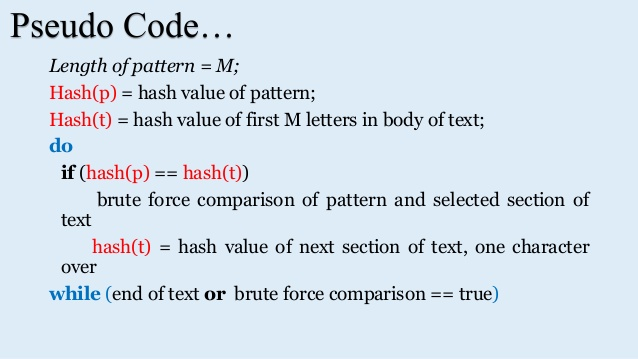
\includegraphics[scale=0.4]{rbpseudo.jpg}
\end{center}
\paragraph{} Pentru implementarea acestei solutii am folosit functia Bernstein, care este una consacrata prin performantele si siguranta care i-au fost demonstrate de-a lungul timpului.

\paragraph{} Algoritmul \textbf{Knuth-Morris-Pratt} cauta potrivirea unui cuvant intr-un text pe baza ideii ca atunci cand se realizeaza o potrivire partiala, cuvantul in sine contine destula informatie astfel incat sa se poata sari peste un anumit numar de caractere despre care se stie ca sunt la fel si in pattern, si in text. Mai precis, functia/tabela specifica acestui algoritm \textit{("failure-function"/"partial match table")}  raspunde la intrebarea "care sufix din potrivirea partiala realizata pana intr-un moment de timp poate constitui un prefix pentru o eventuala potrivirire ulterioara?".
\paragraph{} Primul pas in implementarea acestei solutii o reprezinta preprocesarea tabelei caracteristice, care presupune:
\begin{itemize}
\item verificarea oricarei secvente din pattern care este identica cu inceputul acestuia, astfel fiind un posibil prefix in cautare
\item punerea in tabela a valorilor care reprezinta cate caractere pot fi sarite in cazul unei potriviri partiale, in functie de pozitia din cuvant la care s-a ajuns
\end{itemize}
\paragraph{} Urmatorul pseudocod ilustreaza aceasta preprocesare:
\begin{center}
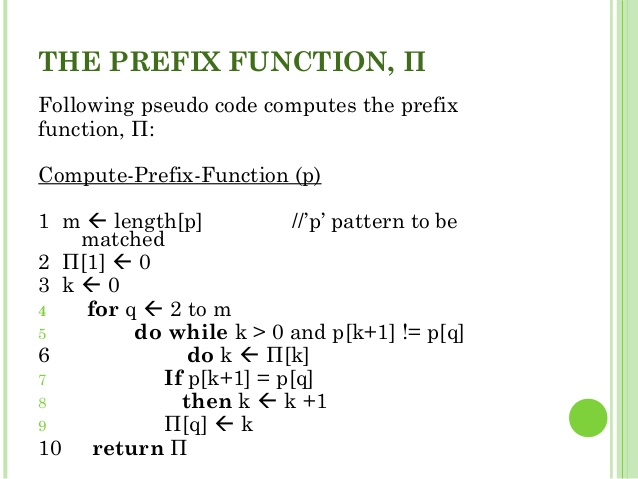
\includegraphics[scale=0.4]{prep.jpg}
\end{center} 
\paragraph{} Partea de cautare este constituita din urmatorii pasi:
\begin{itemize}
\item crearea tabelei caracteristice pentru pattern-ul dat
\item parcurgerea efectiva a textului si verificarea caracter cu caracter cu doi indici diferiti a cate unui caracter din text cu unul din pattern
\item in cazul unui caracter care se potriveste, se parcurg ambele in continuare. Se verifica ca nu s-a ajung la finalul pattern-ului, caz in care a fost gasita o potrivire in text. Aceasta ori se poate adauga intr-o lista sau se poate intoarce indexul unde a fost gasita potrivirea, daca asta se doreste.
\item in cazul unui caracter care nu se potriveste, se revine cu indicele care parcurge pattern-ul pe ultima pozitie indicata de tabela folosita, si se revine la potrivirea caracter cu caracter din acest punct
\item repetarea pasilor de mai sus pana la ultima pozitie de la care poate fi gasit pattern-ul in text
\end{itemize}
\pagebreak
\paragraph{} Urmatorul pseudocod implementeaza aceasta cautare:
\begin{center}
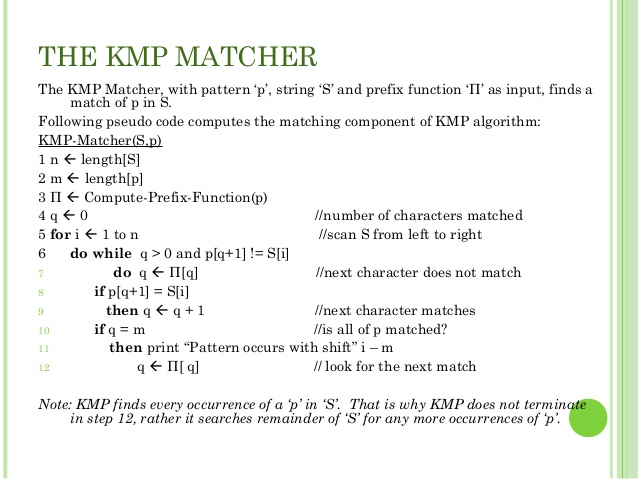
\includegraphics[scale=0.4]{match.jpg}
\end{center}

\subsection{Analiza complexitatii solutiilor}
\textit{Consideram lungimea textului = n si lungimea patternului = m} 

	 	\textbf{Rabin-Karp}  \\
	 	\textit{timp} 
	 	\begin{itemize}
	 		 	\item worst-case: O(nm)
	 			\item best-case: O(n+m) (la fel si pentru average-case)
	 	\end{itemize}
		\textit{memorie} - neglijabil \\

		\textbf{Knuth-Morris-Pratt} \\ 
		 \textit{timp}
		 \begin{itemize}
		 \item cautare: O(n) 
		 \item pre-procesare: O(m) 
		 \item overall: O(n+m)  
		 \end{itemize}
		 		 		 \textit{memorie}
		 \begin{itemize}
		 \item O(m) \\
		 \end{itemize}

\subsection{Principalele avantaje si dezavantaje pentru fiecare solutie}
\textbf{Rabin-Karp} \\
\textit{avantaje} 
\begin{itemize}
\item poate detecta foarte usor plagiarismul pentru ca rezolva foarte bine potrivirile multiple
\item nu este mai rapid ca bruteforce in teorie, dar in practica are complexitate de timp mai buna
\item cu o functie de hashing buna, poate fi destul de eficient si usor de implementat
\end{itemize}
\textit{dezavantaje}
\begin{itemize}
\item sunt multiple solutii pentru aceasta problema care sunt mai rapide decat O(m+n) (unde m este lungimea patternului si n este lungimea textului in care se cauta)
\item este la baza la fel de incet ca bruteforce si necesita si spatiu in plus
\end{itemize}
\textbf{Knuth-Morris-Pratt} \\
\textit{avantaje}
\begin{itemize}
\item are timpul de rulare foarte bun comparativ cu alti algoritmi asemanatori
\item nu are nevoie sa se miste inapoi in textul dat, astfel fiind foarte eficient in procesarea fisierelor de dimensiuni mari
\end{itemize}
\textit{dezavantaje}
\begin{itemize}
\item nu functioneaza asa de bine odata cu cresterea dimensiunii alfabetului folosit deoarece creste posibilitatea unei potriviri gresite
\end{itemize}

\section{Evaluare}
\subsection{Construirea setului de teste}
\paragraph{} Am considerat ca un numar prea mic de teste nu este relevant pentru a vedea comportamentul celor doi algoritmi in totalitate. Cele 30 de teste create se impart in mai multe categorii: \\
\begin{itemize}
\item 1 - 5: text de dimensiune scurta cu o singura potrivire 
\item 6 - 10: text de dimensiune scurta cu nicio potrivire 
\item 11 - 15: text de dimensiune medie cu multiple potriviri 
\item 16 - 20: text de dimensiune medie cu nicio potrivire 
\item 21 - 25: text de dimensiune mare cu multiple potriviri 
\item 26 - 30: text de dimensiune foarte mare cu multiple potriviri sau niciuna 
\end{itemize}
\paragraph{In crearea testelor am incercat sa fiu cat mai variat pentru a intelege cat mai bine comportamentul algoritmilor in speta, asa ca am inclus de la carti intregi ("Hobbitul" - copiat de 2 ori pentru ca parea cam scurt, multiple carti ale lui Jules Verne in acelasi test, "Povestea lui Harap-Alb" si altele) pana la primul milion de zecimale ale lui pi, sau un sir de zeci de milioane de numere generate random.}

	
\subsection{Specificatiile sistemului de calcul}
CPU: 2,6 GHz 6-Core Intel Core I7 \\
RAM: 16GB 2400MHz DDR4 \\
Disk: 500GB SSD \\
GPU: 1,5GB Intel UHD Graphics 630 / 4GB Radeon Pro 560x \\
OS: MacOS Catalina 10.15.1 \\

\subsection{Rezultatele evaluarii solutiilor pe setul de date}
\paragraph{} In urma rularii celor doi algoritmi pe setul de date construit, in majoritatea cazurilor timpii obtinuti au fost foarte asemanatori, variatiile fiind constante pentru toate testele. Am realizat o medie a timpilor de rulare (cu ajutorul unui script) pentru 10 rulari diferite, valorile aproximate fiind urmatoarele:
\begin{center}
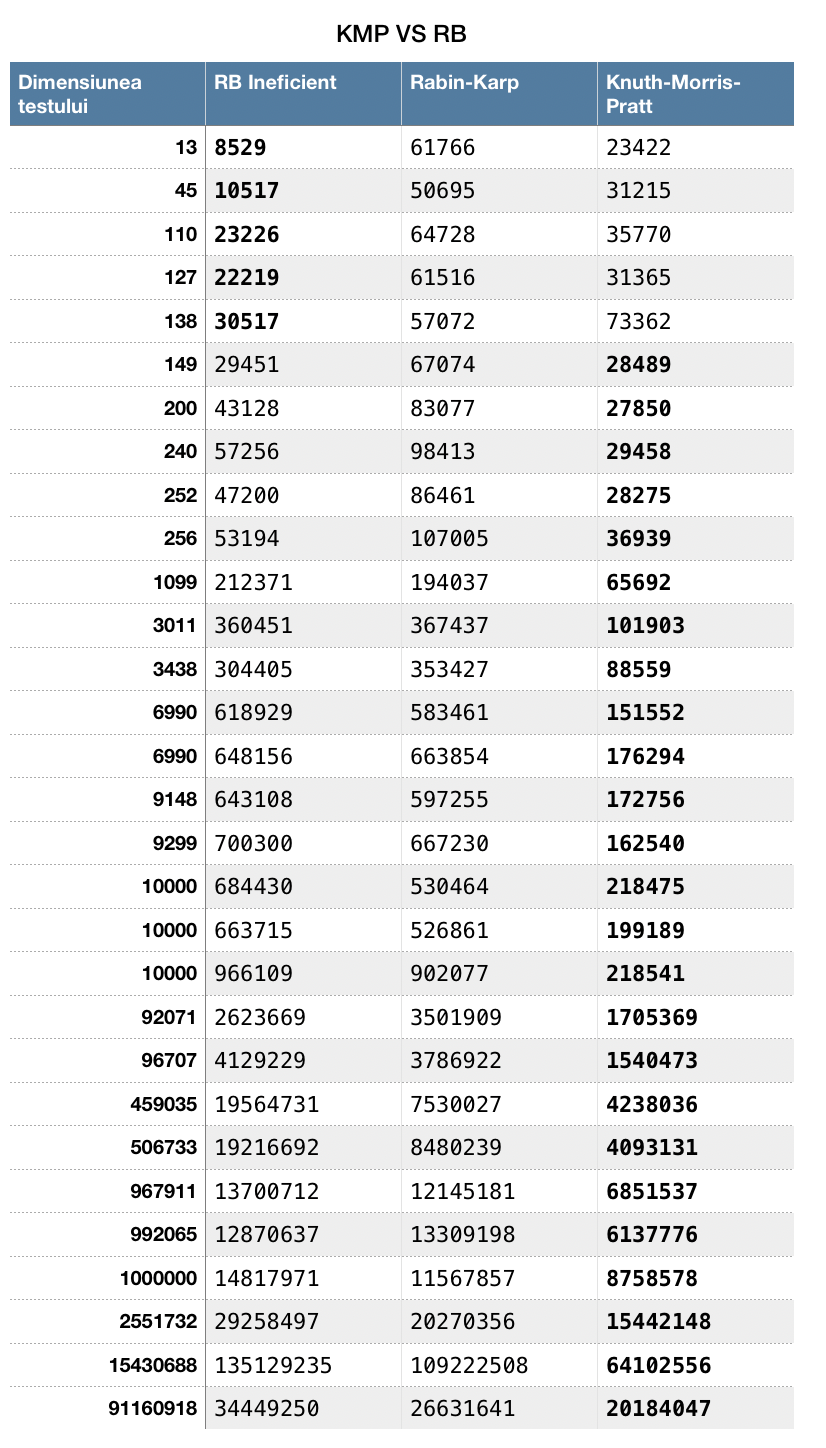
\includegraphics[scale=0.5]{rezultate.png} \\
\end{center} 
\paragraph{} \textit{Observatii:} 
\begin{description}
\item [Dimensiunea testului] reprezinta numarul de caractere (bytes) pe care il are textul in care se realizeaza cautarea pattern-ului.
\end{description}
\paragraph{} Urmatoarele trei coloane reprezinta timpii de rulare (in nanosecunde) pentru trei puncte de interes ale acestui studiu:
\begin{description}
\item Coloana \textbf{RB Ineficient} corespunde rularii algoritmului Rabin-Karp folosind o functie ineficienta din punctul de vedere al performantei.
\item Coloana \textbf{Rabin-Karp} corespunde rularii algorimului Rabin-Karp folosind o functie consacrata si eficienta (functia Bernstein) din punctul de vedere al performantei.
\item Coloana \textbf{Knuth-Morris-Pratt} corespunde rularii algoritmului Knuth-Morris-Pratt. \\
\end{description}

\begin{center}
Rularea algoritmului Rabin-Karp cu\\ o functie ineficienta vs. o functie eficienta de hashing\\
\end{center}
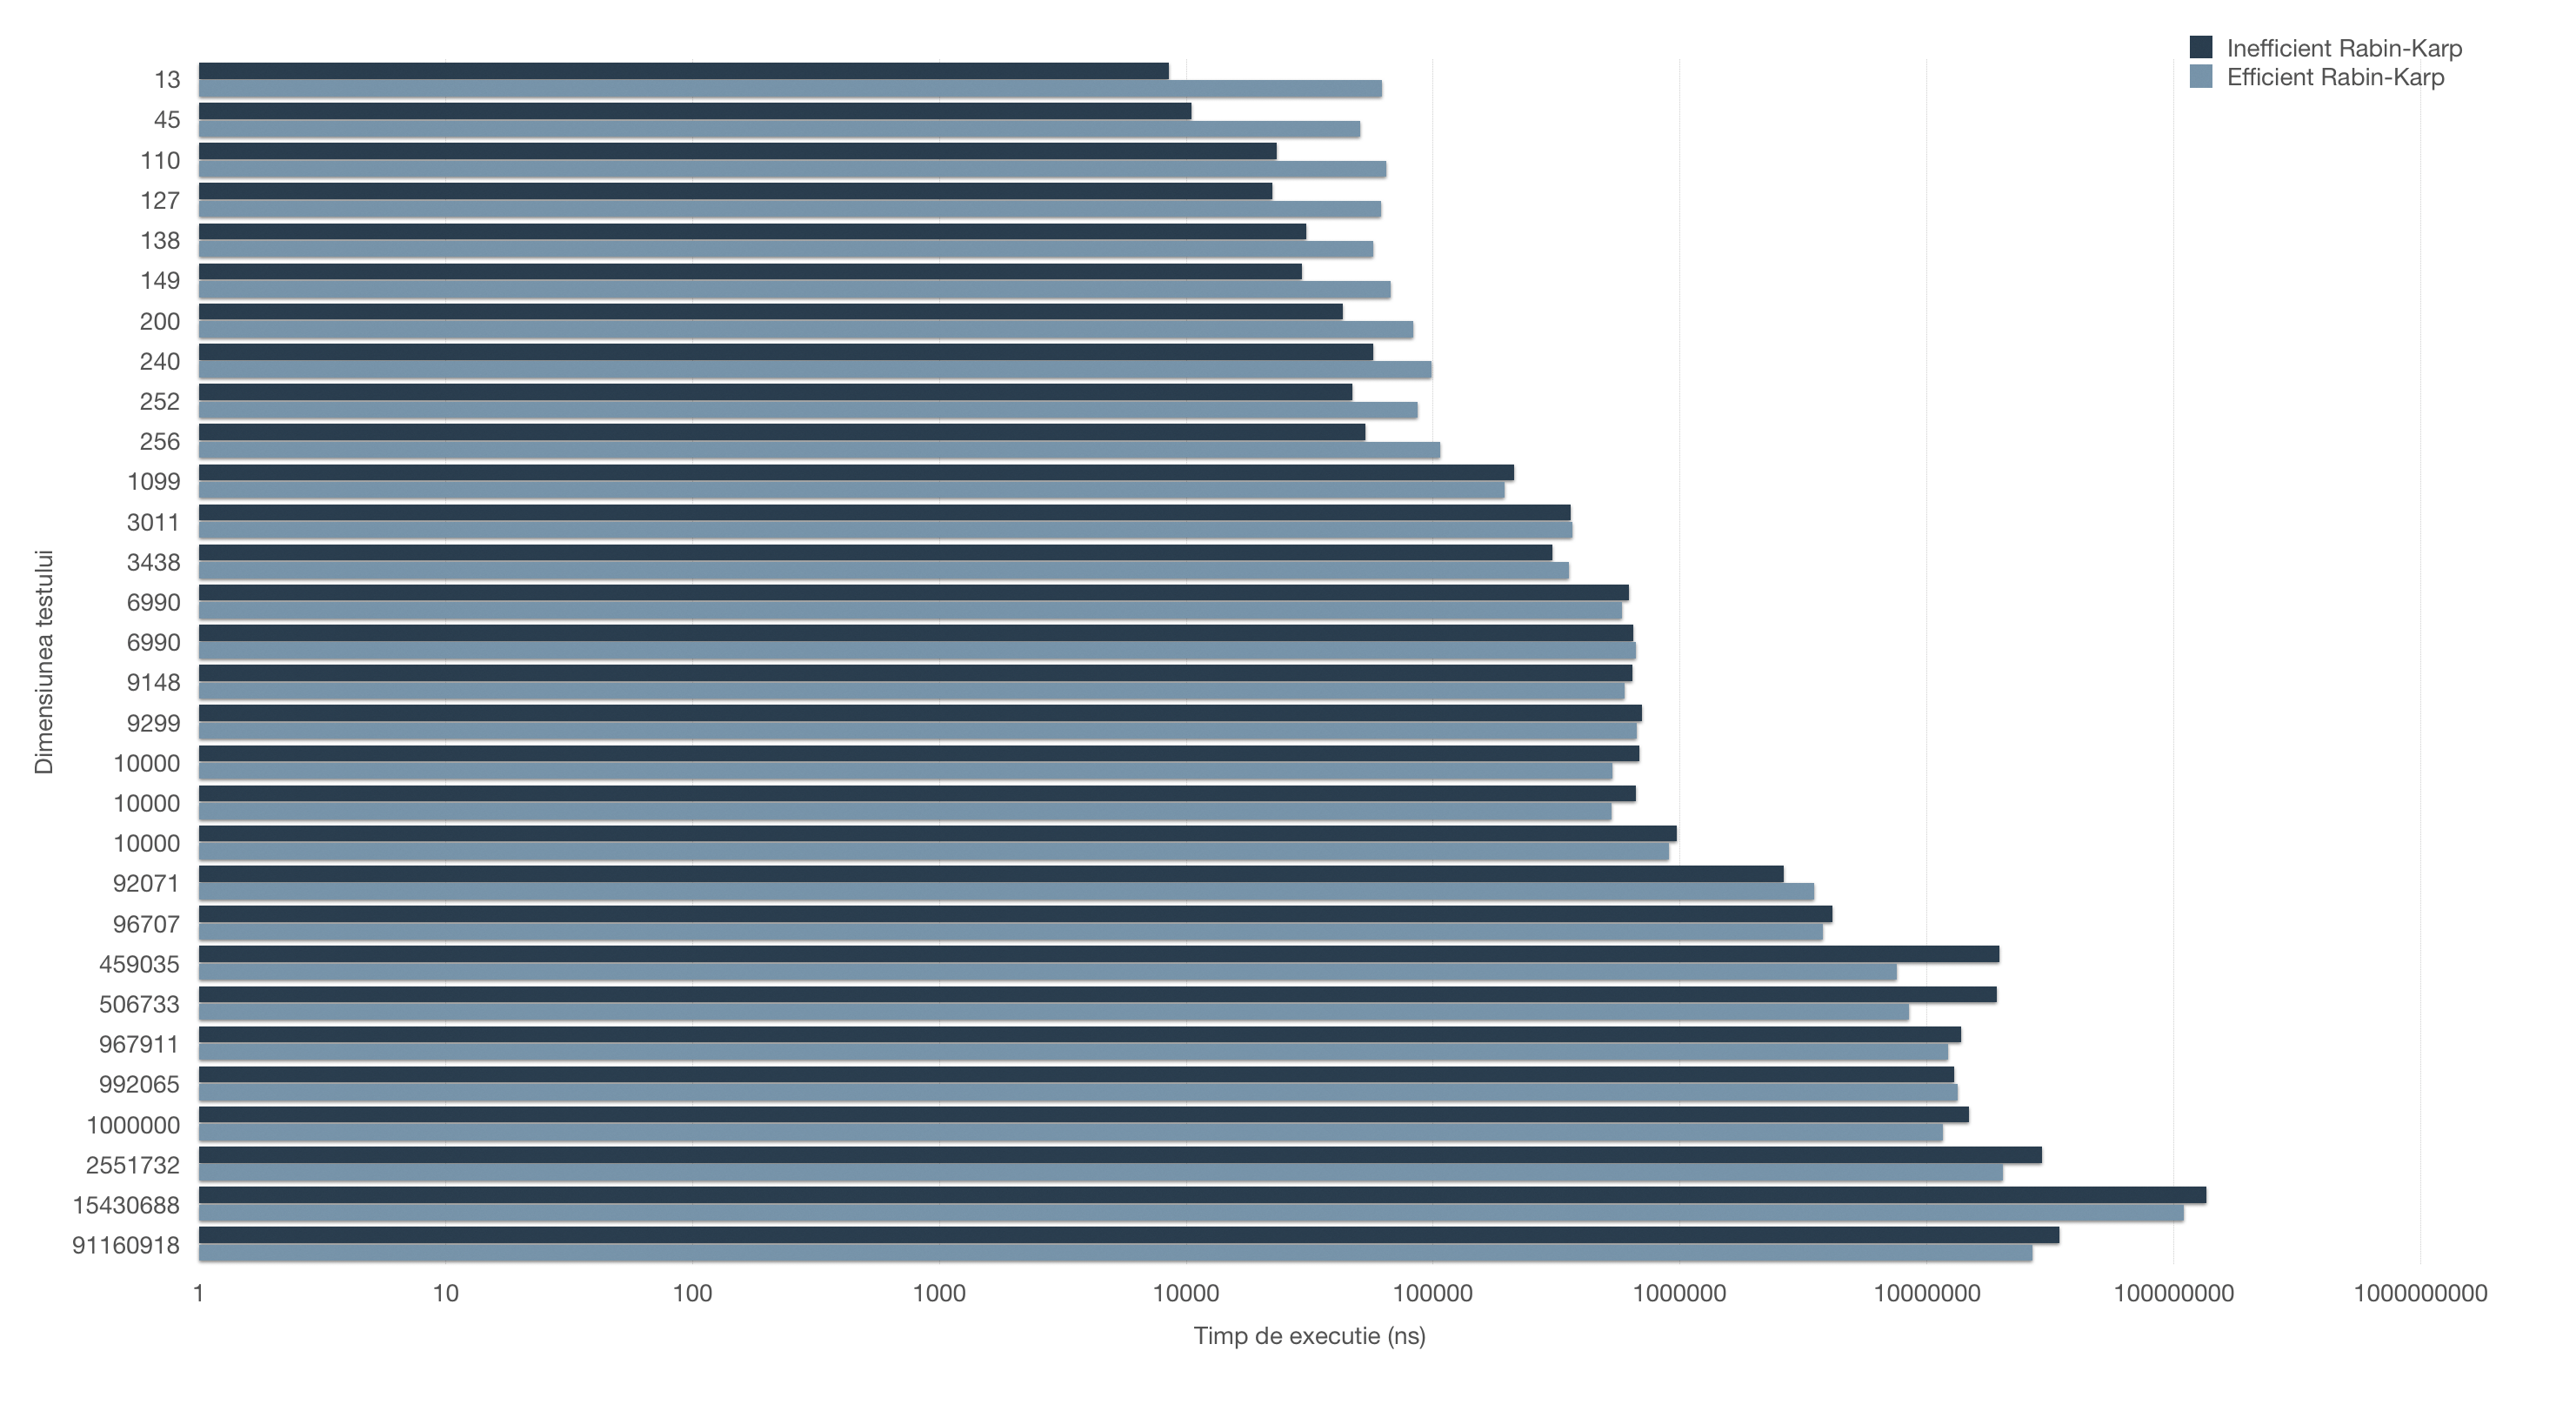
\includegraphics[scale=0.3]{rbvsrb.png}

\pagebreak
\begin{center}
Rularea algoritmului \\ Rabin-Karp cu functia Bernstein vs. algoritmul Knuth-Morris-Pratt
\end{center}
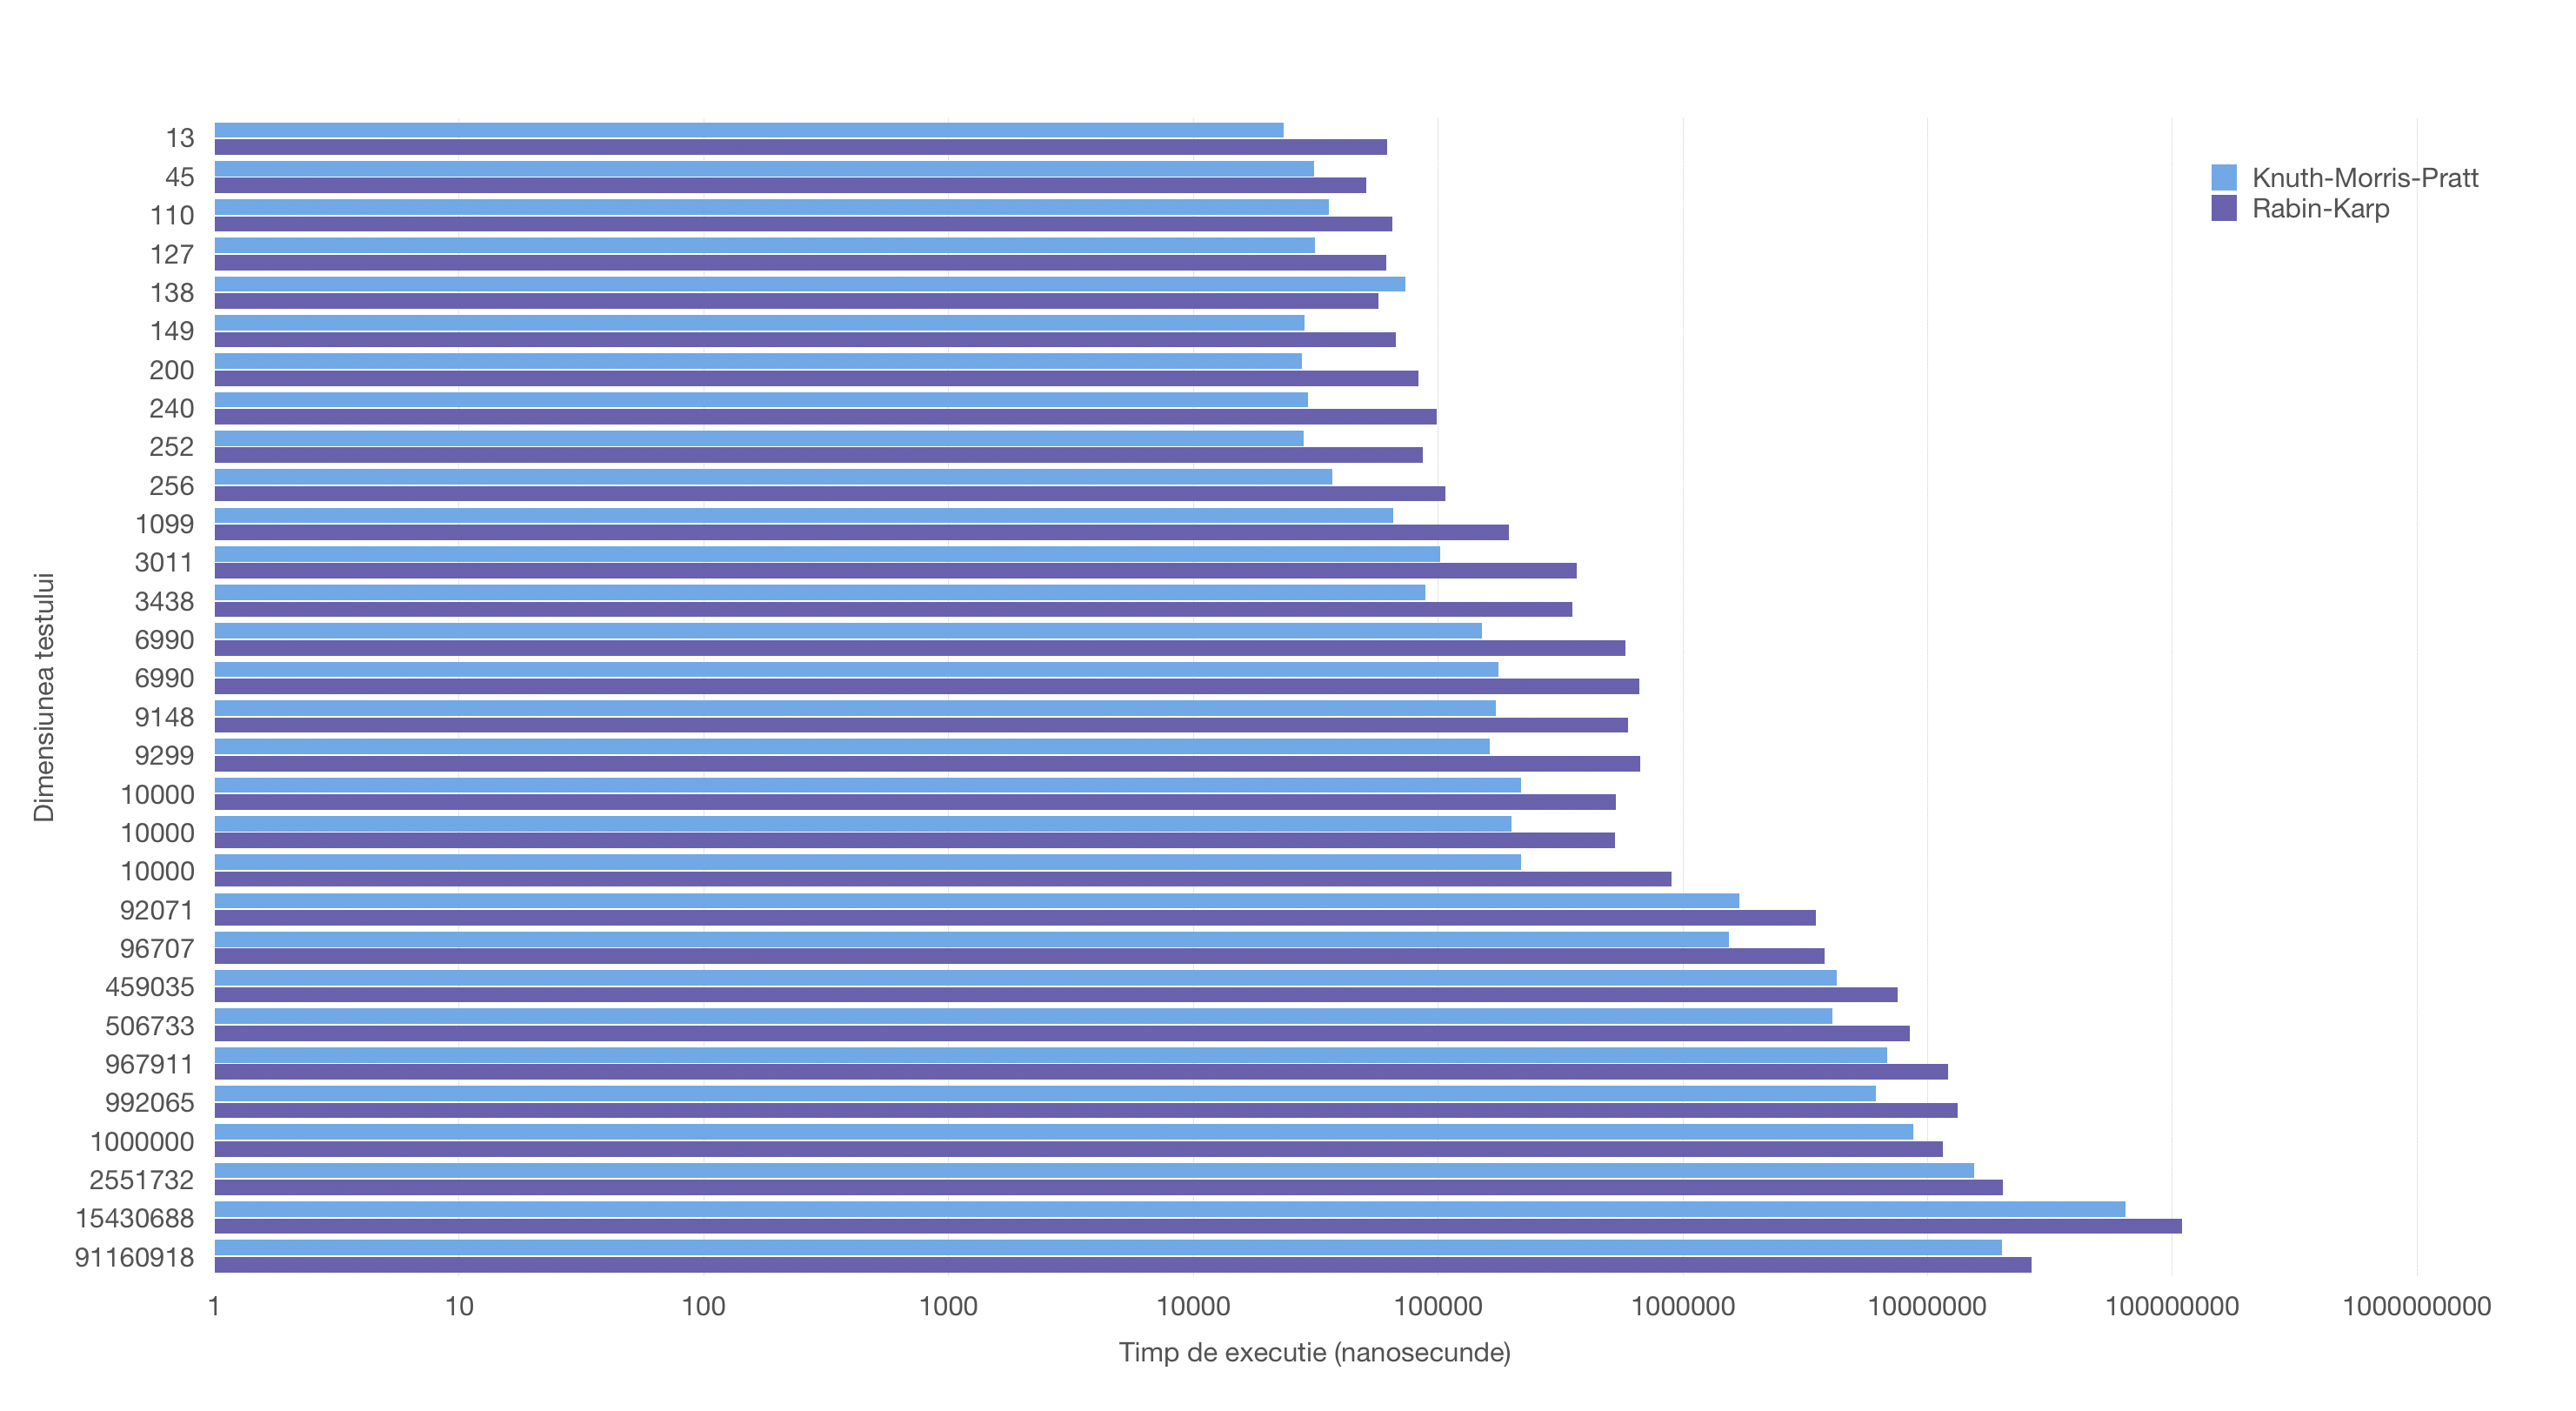
\includegraphics[scale=0.3]{rbvskmp.png}

\par \textbf{Observatie:} Timpul de rulare este masurat strict pentru partea caracteristica algoritmului. Citirea datelor si scrierea rezultatelor nu intra in acest timp. \\

\par \textbf{Observatie:} Timpul de rulare se doreste a fi cat mai mic. Un timp mai mic de rulare inseamna eficienta sporita. \\

\par \textbf{Observatie:} Scara folosita pentru ilustrarea timpilor de rulare in cele doua grafice de mai sus este una logaritmica. Am considerat acest lucru deoarece folosind una liniara nu se putea vedea atat de clar diferenta pe acelasi grafic a testelor de dimensiuni mari si a celor de dimensiuni mici din cauza diferentei timpilor obtinuti. De asemenea, un aspect important de tinut minte in continuare este acela ca orice mica diferenta intre doua valori care este pe grafic este in realitate mult mai  decat pare.

\subsection{Prezentarea valorilor obtinute pe teste}
\paragraph{Rularea algorimului Rabin-Karp cu doua functii diferite de hashing} duce la un numar de valori surprinzatoare deoarece in anumite cazuri, rularea algoritmului Rabin-Karp cu functia ineficienta se aseamana foarte mult cu cea eficienta, chiar fiind mai rapida in anumite teste. Acest fapt poate avea mai multe cauze: 
\begin{itemize}
\item Cauza principala este faptul ca pattern-ul este de o lungime mica.
Faptul ca folosind functia ineficienta se parcurg efectiv toate grupurile de lungimea pattern-ului prezente in text nu face nicio diferenta, sau aproape niciuna.
\item Functia Bernstein are si o inmultire pe langa adunarea pe care o are si cealalta functie.
\end{itemize}
\paragraph{} De asemenea, acest aspect apare din ce in ce mai putin cu cat dimensiunea
	textului este mai mare. Asta deoarece creste diferenta dintre a parcurge
	pattern-ul doar cand valoarea hash Bernstein este aceiasi pentru doua
	siruri de caractere si atunci cand se parcurge pattern-ul efectiv la fiecare
	pas din parcurgerea textului.
	\paragraph{} Nu exista o descriere clara a acestui comportament, dar reprezinta o caracteristica secundara interesanta pentru acest algoritm.
\\ 

\paragraph{Comparand direct cei doi algoritmi vizati de acest studiu} se poate observa ca in majoritatea cazurilor Knuth-Morris-Pratt este mai rapid. Exceptie face un singur test, dar care este de dimensiune prea mica pentru a putea fi luat ca exemplu clar ca Rabin-Karp are cazuri clare cand este mai eficient.
\paragraph{} Acest rezultat se datoreaza faptului ca Rabin-Karp trebuie sa parcurga pattern-ul de fiecare data cand crede ca acesta a fost gasit in textul dat. In cazul celeilalte solutii, potrivirea este realizata fara alte apeluri de functii sau parcurgeri suplimentare.
\paragraph{} Este adevarat ca algoritmul Knuth-Morris-Pratt are si o parte de preprocesare (producerea tabelei specifice), dar in cronometrarea testelor am inclus aceasta parte in timpul total al algoritmului. Astfel, chiar si cu aceasta aditie fata de cealalta solutie, timpii de rulare sunt clar mai buni.

\section{Concluzii}
\paragraph{} Algoritmul Knuth-Morris-Pratt este mai eficient in majoritatea cazurilor, performanta lui fiind, de asemenea, direct proportionala cu dimensiunea problemei abordate.

\subsection{Abordarea problemei in practica}
\paragraph{} Algoritmul \textbf{Rabin-Karp} ar trebui ales in cazurile in care cuvantul sau secventa care trebuie cautata se preconizeaza sa fie gasita de mai multe ori in text (cautarea/verificarea plagiatului, de exemplu).
\paragraph{} Algoritmul \textbf{Knuth-Morris-Pratt} ar trebui ales in cazurile in care problema presupune cautarea intr-un text de dimensiuni foarte mari sau atunci cand pattern-ul in sine are foarte multe secvente repetitive identice cu una de inceput.

\pagebreak
\begin{thebibliography}{8}
\bibitem hhttps://www.cs.auckland.ac.nz/courses/compsci369s1c/lectures/GG-notes/CS369-StringAlgs.pdf \\
\bibitem hhttps://www.slideshare.net/sabiyasabiya/knuth-morris-pratt-string-matching-algo-85219763 \\
\bibitem hhttps://www.javatpoint.com/computer-network-routing \\
\bibitem hhttps://academic.oup.com/bioinformatics/article-abstract/9/3/299/225240 \\
\bibitem hhttps://docs.lib.purdue.edu/cgi/viewcontent.cgi?article=2115\&context=cstech \\
\bibitem hhttps://www.researchgate.net/publication/2432009\_Pattern\_Matching\_Techniques\_and\_Their\_Applications\_to\_Computational\_Molecular\_Biology\_-\_A\_Review \\
\bibitem hhttps://dzone.com/articles/algorithm-week-rabin-karp \\
\bibitem hhttps://www.slideshare.net/GajanandSharma1/rabin-karp-string-matching-algorithm \\
\bibitem hhttps://www.slideshare.net/alokeparnachoudhury/string-matching-algorithm \\
\bibitem hhttps://brilliant.org/wiki/rabin-karp-algorithm/ \\
\bibitem hhttps://brilliant.org/wiki/knuth-morris-pratt-algorithm/ \\
\end{thebibliography}
\paragraph{Toate site-urile care au fost referentiate mai sus au fost ultima data accesate in data de 13 decembrie 2019.}
\end{document}
